\documentclass[12pt,a4paper, dvipsnames,usenames]{article}
\setlength{\textwidth}{165mm}
\setlength{\textheight}{240mm}
\setlength{\parindent}{0mm} % S{\aa} meget rykkes ind efter afsnit
\setlength{\parskip}{\parsep}
\setlength{\headheight}{0mm}
\setlength{\headsep}{0mm}
\setlength{\hoffset}{-2.5mm}
\setlength{\voffset}{0mm}
\setlength{\footskip}{15mm}
\setlength{\oddsidemargin}{0mm}
\setlength{\topmargin}{0mm}
\setlength{\evensidemargin}{0mm}
\usepackage{graphicx}    % For grafik (billederfiler)
\usepackage[T1]{fontenc} % For at blande \textsc{} med \textbf{}
\usepackage[utf8]{inputenc}
\usepackage{capt-of}
\usepackage{caption}
\usepackage{amsfonts,amsmath,amssymb}
\usepackage{eucal}

\usepackage{algorithm}
\usepackage{algpseudocode}

\usepackage{listings}
\usepackage{pdfpages}
\usepackage[english]{babel}
\usepackage{enumerate}
\usepackage[utf8]{inputenc}
\usepackage{url}
\usepackage{multirow}
\usepackage{color}
\usepackage{cite}
\usepackage{mathtools}
\usepackage{pdfpages}
\usepackage{enumitem}
\usepackage{minted}
\definecolor{KU-red}{RGB}{144,26,30}
\definecolor{dkgreen}{rgb}{0,0.6,0}
\definecolor{gray}{rgb}{0.5,0.5,0.5}
\definecolor{mauve}{rgb}{0.58,0,0.82}
%% color for background of code listing
\definecolor{bg}{rgb}{0.95,0.95,0.95}
\usepackage{hyperref}
\usepackage{natbib}
\hypersetup{
    colorlinks,
    citecolor=black,
    filecolor=black,
    linkcolor=black,
    urlcolor=black
}
\lstset{%
  breaklines=true,
  breakatwhitespace=true,
}
\usepackage[noabbrev,nameinlink]{cleveref}  % Cleveref must be loaded after hyperref.
\usepackage{enumitem}

% hack for minted
\AtBeginEnvironment{minted}{\dontdofcolorbox}
\def\dontdofcolorbox{\renewcommand\fcolorbox[4][]{##4}}

% fix unicode
\DeclareUnicodeCharacter{207B}{⁻}

%%====================================================================
%% Main document
%%====================================================================

\begin{document}

%%% Header
\begin{minipage}[b]{1.0\linewidth}

\includegraphics[height=30mm]{KULogo.pdf}
\vspace*{-16ex}
\begin{center}
  {\large \bf PAT Final Assignment: \\ Automatic Function Inversion in Haskell}
  \vspace*{2ex} \\
\vspace*{1ex}
Klaus Philipp Theyssen - lwg303
\end{center}
\vspace {1ex}
\vspace*{-8pt}
{\color{KU-red}\hrule}
\end{minipage}

\section*{Abstract}

Function inversion is an important concept and can be used to save time
and avoid bugs. Applications are for example compression/decompression and
encryption/decryption algorithms. Using a reversible language like
Janus, the programmer gets inverse functions for ``free''.
In this work I discuss a specific method for automatic function inversion in Haskell
implemented via a GHC plugin. Haskell has a larger user base
than Janus and is also used in industry. Therefore, exploring automatic
function inversion in Haskell gives insight into how
automatic inversion can be applied outside research.
First I explain in broad terms the approach used by the GHC plugin
to generate inverses. Finally, I present results from
implementing various algorithms, discussing limitations and benefits of the plugin.



\section{Introduction}

\subsection{Motivation}

As we have seen in the course, function inversion
is a powerful concept, which can help during software development.
It can save time by avoiding having to implement inverse functions
and preventing bugs, for example in compression algorithms.
In the lectures we have seen function inversion in the setting of Janus,
which is a research project focused on reversible computation. Trying to bring
some of the benefits of function inversion to a mature system like Haskell is a
worthwhile endeavor. Haskell has seen increasing adoption in industry and
is used at large companies like Facebook (\cite{marlow2013haxl}).

\subsection{Goals of Work}

The goal of this work is two-fold. First I want to make the work from
\cite{teegen2021haskell} more accessible, as it is mostly focused on the
implementation details of the automatic inversion framework related to Haskell.
I on the other hand want to emphasize the underlying
idea for generating the inverse functions.

Secondly I want to give an outlook on the usability and benefits one might
get from using the plugin and also discuss its shortcomings.


\subsection{Summary of contributions}
The contribution of this work is giving a high-level summary of
the approach for automatic function inversion presented in \cite{teegen2021haskell},
skipping the technical details related to Haskell.

Further I implemented various modules in Haskell using the plugin,
measuring the performance of the generated inverses and also giving a short account
of my experience using the plugin.

The remainder of this report is organized as follows:

\begin{itemize}
\item \textbf{Section 2:} In this section I talk about inversion in the setting
of functional languages in general. For this, I review and discuss various approaches
from the literature.

\item \textbf{Section 3:} Here I present the fundamental idea of the
  inversion framework using a functional-logic extension of Haskell.

\item \textbf{Section 4:} Evaluating the GHC Plugin, its usability and performance,
  by implementing various algorithms and small programs.

\item \textbf{Section 5:} In this part I give a short conclusion and discuss
  various other ideas to explore, but also limitations of my own work.
\end{itemize}


\section{Inversion in Functional Languages}

In this section, I want to review the literature on inverting functional languages.
In the PAT course we have seen the imperative reversible language
Janus.

The Universal Resolving Algorithm introduced in \cite{abramov2000universal},
performs inverse computation for first-order functional
languages and is based on perfect process trees.
In \cite{abramov2007universal} the URA has
been extended to lazy functional languages.

A different kind of approach is to design a reversible functional language
from the ground up. This has been
explored in \cite{yokoyama2012towards} and \cite{mu2004}.
If we only consider injective functions, one
can use techniques from LR parsing to generate
inverses as presented in \cite{gluck2004LR}.

In \cite{teegen2021haskell} the authors do not limit themselves to
injective functions, which would be impractical for  a general purpose
language like Haskell. Instead they employ
techniques from logic programming languages like Prolog, in order to provide
inverses via non-determinism. Therefore, the generated inverse
functions return a list of possible results.
This idea is closely connected to functional-logic programming languages like
Curry (see \cite{Hanus2013Curry}).


\section{Approach to Automatic Function Inversion in Haskell}

The core concept of the plugin is utilizing free-variables and non-determinism
in order to generate inverses. This is done by extending Haskell computational
model to a functional-logic computational model using Monads.
All functions, constructs and expressions of a Haskell module
are lifted into the Monad.

Thus, the underlying inverse computation is similar to that of
logic programming languages like Prolog, where one can call predicates
with free variables as arguments to find
variable bindings such that the predicate is satisfied.
For example in Prolog we can do the following:

\begin{minted}[breaklines]{prolog}
prolog> append(Xs, Ys, [17,42]).
Xs = [], Ys = [17, 42] ;
Xs = [17], Ys = [42] ;
Xs = [17, 42], Ys = [] ;
false.
\end{minted}

\subsection{Functional-logic extension of Haskell}

The functional-logic extension is realized using free variables and non-determinism.
The free variables are implemented with
identifiers and a heap, which keeps track of already
instantiated free variables in each computational branches.
In addition, non-determinism is modeled via multiple computation branches
using a tree. The tree and its different computational
branches are explored in a breadth-first manner, in order to avoid getting
stuck in an infinite computation of a single computation branch.
Since most general purpose functions written in Haskell are non-injective,
the inverses return a list of possible results.
Further, this approach lends it self easily to implemented partial inverses,
we can simply provide the additional fixed arguments instead of using free variables.
The steps for computing the automatic inverses is described in
\cref{fig:inversion-steps}.

\begin{figure}[h]
\fbox{
\parbox[c]{\textwidth}{
\centering
\begin{enumerate}
\item Lift function (type, definition + expressions) into functional-logic computational model (Monad) including following transformations:
  \begin{itemize}
  \item simplify pattern matching into unary lambda abstraction
  \item non-exhaustive pattern augmented with pattern match failure
  \end{itemize}

\item Run lifted function, with free variables as arguments (Heap keeps track
  of instantiated free variables)

\item During computation pattern matching leads to instantiation of free variables
  (narrowing), where for each constructors of the datatype a
  new computation branch is spawned

\item Evaluate to ground normal form to ensure result does not contain free variables

\item Match results of functional-logic computation with argument
  for inverse function. For each matching computation branch we
  get one result for the inverse computation
  (the value the arguments have been instantiated to)
\end{enumerate}
}}

\caption{Steps of Inversion Framework}
\label{fig:inversion-steps}
\end{figure}

\subsection{Example: Inverse Generation for List Concatenation}

To illustrate the approach of the plugin, I want to give a high level
overview how the inverse of the list concatenation function \texttt{(++)}
is generated.
\begin{minted}[breaklines]{haskell}
(++) :: [a] -> [a] -> [a]
[] ++ ys = ys
(x:xs) ++ ys = x : xs ++ ys
\end{minted}
As the plugin uses template haskell \cite{sheard2002template}, we can easily
define the inverse function \texttt{split} by referring to the original function as follows: \begin{minted}[breaklines]{haskell}
split :: [Int] -> [([Int], [Int])]
split = $(inv '(++))
\end{minted}
In a \textbf{ghci} session we can do the following:
\begin{minted}[breaklines]{Haskell}
*Main> split [17,42]
[([],[17,42]),([17],[42]),([17,42],[])]
\end{minted}
An example for how the steps from \cref{fig:inversion-steps}
create various
computation branches and finally the result of the inverse computation is
shown in \cref{fig:inverse-comp}.

\begin{figure}[h]
\begin{minipage}{1.0\linewidth}
  \begin{center}
    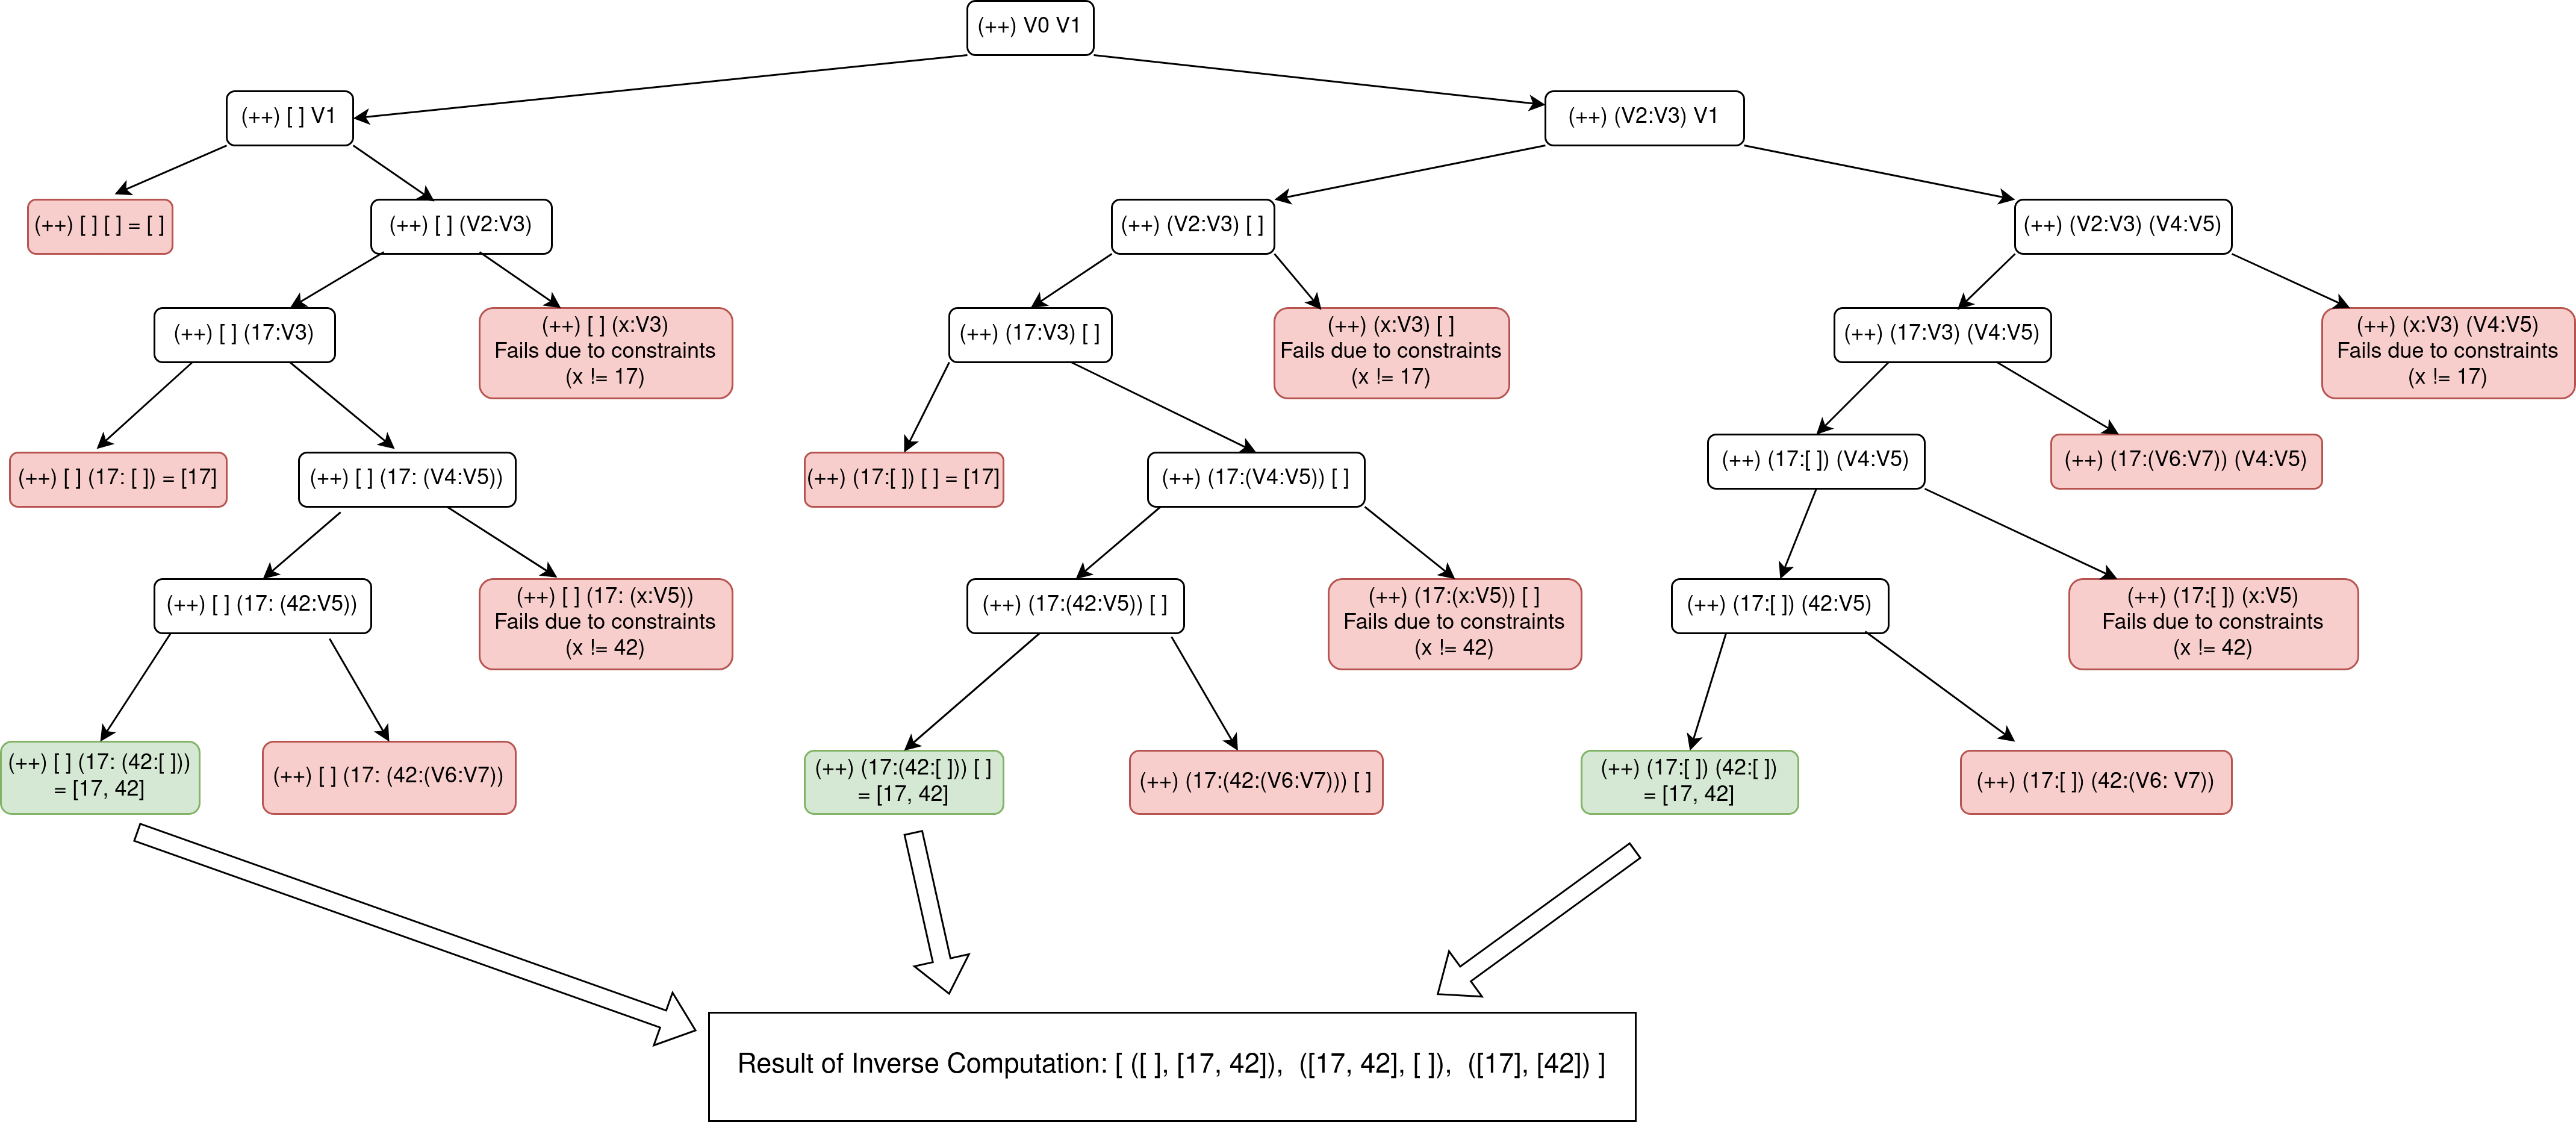
\includegraphics[scale=0.115]{resources/inverse-computation-drawing.png}
    \caption{
      Drawing of example inverse computation: \texttt{split [17,42]}.
      At each arrow the value of the next free variable is instantiated
      to all possible values according
      to the constructor of the data type.
      For the list data type this is either [ ] or $(V':V'')$. For the primitive
      data type Int constraints are used (see \cref{sec:prim}). Further we see
      that only computation branches are matched, for which the result of the lifted
      function is equal to the argument of the inverse function.
    }
     \label{fig:inverse-comp}
  \end{center}
\end{minipage}
\end{figure}

\subsection{Primitive types}
\label{sec:prim}

Dealing with primitive types like integers is not easy, because in order
to instantiate free variables the implementation pattern matches on the constructors
of the type. In the case of integers a computation branch would be spawned
for each of the 
$2^{64}$ possible values. To circumvent this, the plugin instead introduces
a constraint each time a pattern-match on a primitive type is made.
For this new constraint the plugin checks if it conflicts with the
previous ones: in case of a conflict the computation branch is terminated, otherwise
it is added to the list of constraints and the computation branch continues.
The constraint solving is implemented using an SMT solver
like Z3 from \cite{Moura2008Z3}.

\subsection{Partial inverses}

The plugin easily allows computing partial inverses.
It is done similarly to regular inverse, but now the
fixed argument is also provided to the lifted function.

As an example consider the following insertAt function:

\begin{minted}[breaklines]{haskell}
insertAt :: Int -> Int -> [Int] -> [Int]
insertAt 0 x xs = (x:xs)
insertAt i x l@(y:ys) =
  case i < 0 of
    True -> error "invalid index"
    False ->
      case i > (length l) of
        True -> error "invalid index"
        False -> y : (insertAt (i-1) x ys)
\end{minted}

Which takes an index, an integer and a list of integers and
inserts the integer into the list at the specified index.

If we now fix its first argument (the index) and compute
its partial inverse, we get a function which
given an index and a list returns the element at that index
and the remaining list after removing the element.

\begin{minted}[breaklines]{haskell}
removeAt1 :: Int -> [Int] -> [(Int, [Int])]
removeAt1 = $(partialInv 'insertAt [1])
\end{minted}


\section{Evaluating the GHC Plugin}
%% Describe implemented examples, compare to other tools
%% ease of use create maybe some chart, measuring performance, code size etc.

First, one has to note that Haskell has a special relation
with language extensions and plugins compared to other programming languages.
Due to the broad use in academia for prototyping new programming language research,
there is a plethora of concepts provided by extensions and
plugins to the Haskell language. Some examples include
Liquid Haskell discussed in \cite{Vazou2016LiquidHH} and
template meta programming as shown in \cite{sheard2002template}.
This is possible because one can add phases in the GHC (Haskell compiler)
and thereby perform additional transformation to the core language
(internal intermediate language of the Haskell compiler).
This leads to a somewhat complex situation of choosing
which plugins and language extension are compatible with each other.
The inversion plugin is for example tied to a specific GHC version (8.10.4).
Being fixed to a specific GHC version, it seems a little bit unrealistic
the plugin can be used in a real world projects, but this is also stated by the
authors in \cite{teegen2021haskell} and natural for a research project.

For evaluating the plugin I implemented various basic algorithms
and functions, which I will discuss in the following.

\subsection{Experiments}

\subsubsection{Free Fall}

First, I implemented the simple free fall simulation (\cref{A:sim})
we have seen in the course, which involves some basic arithmetic.
This was very straightforward and generating the inverse succeeded
on the first try.

\subsubsection{Run Length encoding}

Next, I moved on to implementing a compression algorithm. I started with
a simple run length encoding algorithm.
During the implementation of this algorithm, I already encountered  some problems,
since the plugin does not work with functions from Haskell's Prelude, and therefore
I had to re-implement various basic list functions in the module like
\texttt{map}, \texttt{head}, \texttt{length} and \texttt{takeWhile}.

\subsubsection{TEA Tiny encryption algorithm}

For an encryption algorithm I chose to implement the
tiny encryption algorithm from \cite{wheeler1995tea}.

After doing some research on how to implement bit manipulations in Haskell, the
packages Data.Bits and Data.Word seemed like the best option.
But it turns out using functions from these packages is not supported
by the plugin.
Whereas for the run length encoder I could re-implement the needed functions on
lists, it was not feasible in this case. Thus, I gave up on generating
inverses with the plugin for the TEA, and
conclude that the plugin is not suited for implementing encryption algorithms
on the bit level in its current form,
except one accepts the extra burden of implementing
basic functions for working with bits using only basic Haskell constructs.

\subsection{Benchmarks}

All the benchmarks were run on a single machine
with a 4-core Intel(R) Core(TM) i5-5200U CPU
processors clocked at 2.20GHz.
The machine has 8GB of DRAM and runs 64-bit Linux 5.13.

For implementing the benchmarks I used the Haskell library
criterion\footnote{\href{https://hackage.haskell.org/package/criterion}{https://hackage.haskell.org/package/criterion}}.


\begin{figure}[h]
\begin{minipage}{1.0\linewidth}
  \begin{center}
    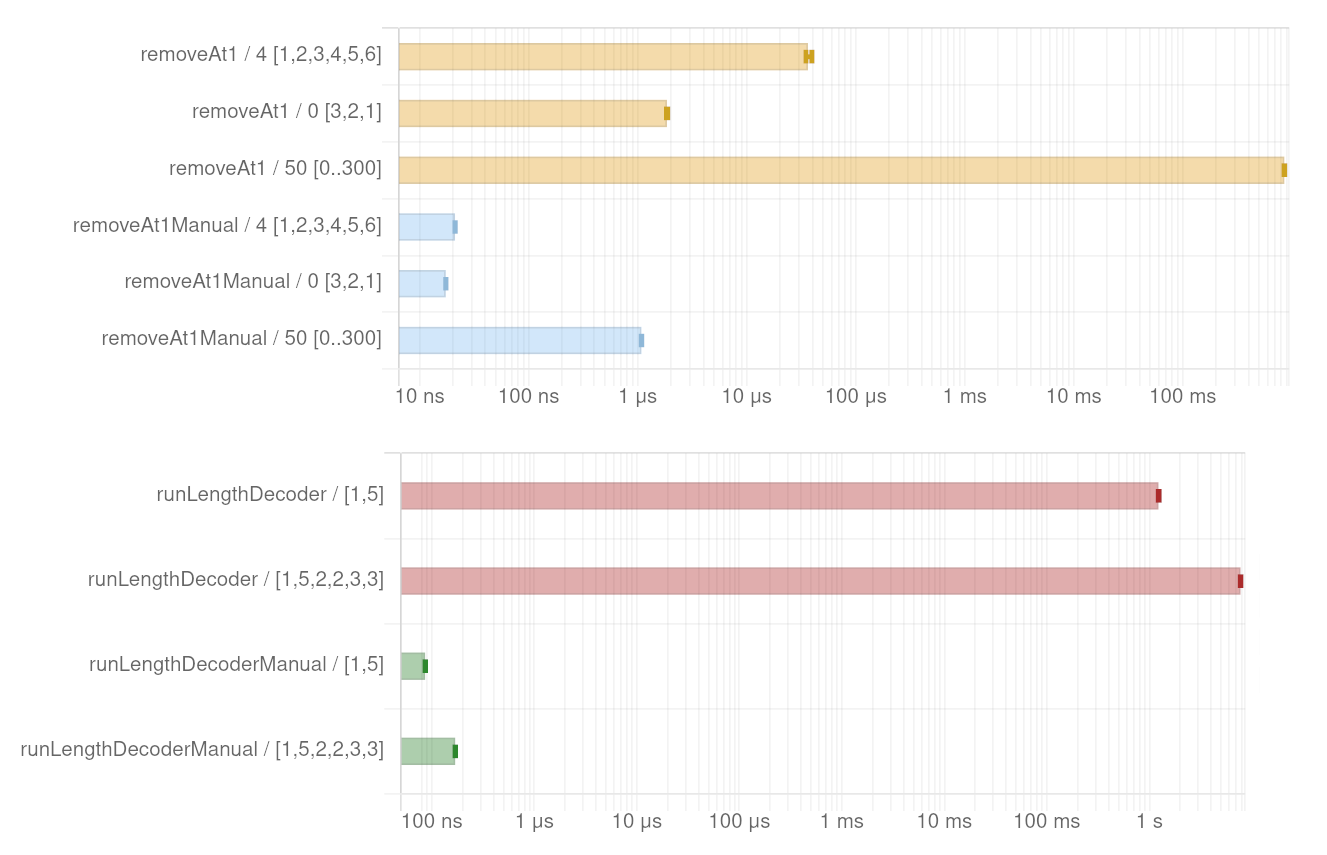
\includegraphics[scale=1.4]{resources/benchmark.png}
     \caption{\small
       {\color{gray!25!black!60} Top:}
       Results from comparing automatic generated removeAt1 (partial inverse)
       function with manual written inverse.
       {\color{gray!25!black!60} Bottom:}
       Results from comparing automatic generated run length decoder
       vs. manual written one.
     }
     \label{fig:bench}
  \end{center}
\end{minipage}
\end{figure}

Each benchmark is run for 5 seconds. The plot shows the mean run time of
all iterations that completed in those 5 seconds.

The x-axis of the plot shows the mean running time in log-scale. The
individual bars, belong to a specific function identified by its
name and the input it received.

Looking at the top plot, which compares the automatically generated
``removeAt1'' with the manually written ``removeAt1Manual'' function,
we see that for smaller inputs the automatic inverse runs
around 1000 times slower, whereas for larger inputs this difference grows
even more.

For the run length decoder its even worse, here the automatically
generated version is around $10^7$ times slower than the manual one.

Still, one has to keep in mind that these benchmarks are not very exhaustive.
In addition, my implementation
of the run length encoder may not be very suited for inversion
with the plugin and one could get a faster decoder by using
a different implementation. Also both benchmarks use the primitive
datatype of integers, which might come at a performance cost
since these have to be handled with constraints as discussed in
\cref{sec:prim}. Nevertheless, the benchmarks show that the generated
inverses are very slowed compared to a manual implementation.
Therefore, they are only suited for special applications like automatic
test case generation as mention in \cite{teegen2021haskell}.

\subsection{Limitations, Problems encountered}

As discussed in the experiments, one of the biggest
problems is not being able to use parts of external
libraries and the prelude. Additionally no I/O operations are allowed, this
is already mentioned in \cite{teegen2021haskell}.
While one of the goals of automatic inversion is to write less code, this limitation
instead causes us to duplicate code.

During my implementation of free fall I also had problems with
type synonyms, where I wanted to do the following:
\begin{minted}[breaklines]{haskell}
type Height = Int
\end{minted}
which resulted in compilation errors.
So, I had to use algebraic datatypes instead:
\begin{minted}[breaklines]{haskell}
data Height = Height Int
  deriving (Show)
\end{minted}

I encountered some obscure GHC error messages
while writing the run length encoder, for example
one of the error messages in \cref{A:error} claims there
is no inverse for \$, but this is just a syntactic construct
for setting parentheses.
Also, while trying to implement a function on lists I got
an internal GHC error, see \cref{A:error}.


\section{Conclusion}

The plugin turns out to be rather impractical for real world usage,
mainly because of the slow performance and limitations on using external
libraries.

Nevertheless, it is very easy to use and illustrates the power of
the Haskell ecosystem and the Glasgow Haskell compiler for extending
the language. It is impressive that one can easily extend
the computational model of Haskell to include logic programming.

\subsection{Further Work}

In the future I would like to do more exhaustive benchmarks and figure
out which properties of functions result in slow inverses.
I would be interested to see what happens if one can avoid integers
and instead use algebraic data types, which might bring a performance boost.

It would have been also really interesting to implement Huffman-compression
using Huffman-trees as another compression algorithm.

In this report I hope I could give some insight into how
the plugin works from a high-level view and illustrate its usage
with experiments.
Unfortunately this work lacks some theoretical depth, first
in explaining exactly all the subtleties of the plugin (Haskell related, type
theoretic, monads etc.) but also the review of other approaches in the literature
for inversion in a functional language is rather shallow. It would be nice
to take more time and go into more detail, but due to time constraints this
work remained rather superficial.
Also, the plugin has additional features not discussed here like functional patterns
and it can also deal with higher order function inverses.

\bibliographystyle{abbrvnat}
\bibliography{bibliography}

%% color for background of code listing
\definecolor{bg}{rgb}{0.95,0.95,0.95}

\appendix
\newpage

\section{Appendix}

\subsection{Compression.hs}
\label{A:comp}

\begin{minted}[bgcolor=bg,
    linenos, breaklines]{haskell}
{-# OPTIONS_GHC -fplugin Plugin.InversionPlugin #-}
{-# OPTIONS_GHC -Wno-incomplete-patterns #-}
{-# OPTIONS_GHC -Wno-overlapping-patterns #-}
module Compression where

import Prelude hiding ((++), map, takeWhile, dropWhile, length, head)

-----------------------------------------------------------
-- Version without prelude functions:
-----------------------------------------------------------
(++) :: [a] -> [a] -> [a]
[] ++ ys = ys
(x:xs) ++ ys = x : (xs ++ ys)

map :: (a -> b) -> [a] -> [b]
map _ []     = []
map f (x:xs) = f x : map f xs

head :: [a] -> a
head (x:_) = x
head [] = error "bad head"

length :: [a] -> Int
length [] = 0
length (x:xs) = 1 + (length xs)

takeWhile               :: (a -> Bool) -> [a] -> [a]
takeWhile _ []          =  []
takeWhile p (x:xs) = case p x of
  True -> x : takeWhile p xs
  False -> []

dropWhile               :: (a -> Bool) -> [a] -> [a]
dropWhile _ []          =  []
dropWhile p xs@(x:xs') = case p x of
  True -> dropWhile p xs'
  False -> xs

splitList :: [Int] -> [[Int]]
splitList [] = []
splitList [x] = [[x]]
splitList l@(x:_) = (takeWhile eqX l) : (splitList (dropWhile eqX l))
  where
    eqX = (\y -> x == y)

mergeLists :: [Int] -> [Int] -> [Int]
mergeLists [] [] = []
mergeLists (x:xs) (y:ys) = [x,y] ++ (mergeLists xs ys)
mergeLists [] y = y
mergeLists x [] = x

runLengthEncoder :: [Int] -> [Int]
runLengthEncoder xs = mergeLists digits times
  where
    subLists = splitList xs
    digits = map head subLists
    times = map length subLists
\end{minted}



%%==============================================================================
%%==============================================================================

\subsection{Encryption.hs}
\label{A:encryp}

\begin{minted}[bgcolor=bg,
    linenos, breaklines]{haskell}
module Encryption where

import Prelude hiding ((++), map, takeWhile, dropWhile, length, head)

import Data.Bits
import Data.Word

------------------------------------------------------------------------------
-- Implementing the tiny encryption algorithms by David Wheeler, Roger Needham
------------------------------------------------------------------------------

-- 128 bit key
data TEAKey = TEAKey {-# UNPACK #-} !Word32 {-# UNPACK #-} !Word32 {-# UNPACK #-} !Word32 {-# UNPACK #-} !Word32
  deriving (Show)


secretKey :: TEAKey
secretKey = (TEAKey  0xdeadbeef 0xdeadbeef 0xdeadbeef 0xdeadbeef)

delta :: Word32
delta = 0x9e3779b9

myData :: Word64
myData = 0xbadf00000000000d

rounds :: Int
rounds = 32

-- Plugin cannot handle Data.Bits, Data.Word :(
teaEncrypt :: TEAKey -> Word64 -> Word64
teaEncrypt (TEAKey k0 k1 k2 k3) v = doCycle rounds 0 v0 v1 where
  v0, v1 :: Word32
  v0 = fromIntegral v
  v1 = fromIntegral $ v `shiftR` 32
  doCycle :: Int -> Word32 -> Word32 -> Word32 -> Word64
  doCycle 0 _ v0 v1 = (fromIntegral v1 `shiftL` 32)
                      .|. (fromIntegral v0 .&. 0xffffffff)
  doCycle n sum v0 v1 = doCycle (n - 1) sum' v0' v1'
    where
      sum' = sum + delta
      v0' = v0 + (((v1 `shiftL` 4) + k0) `xor` (v1 + sum') `xor` ((v1 `shiftR` 5) + k1))
      v1' = v1 + (((v0 `shiftL` 4) + k2) `xor` (v0 + sum') `xor` ((v0 `shiftR` 5) + k3))
\end{minted}




%%==============================================================================
%%==============================================================================


\subsection{Simulation.hs}
\label{A:sim}

\begin{minted}[bgcolor=bg,
    linenos, breaklines]{haskell}
{-# OPTIONS_GHC -fplugin Plugin.InversionPlugin #-}
{-# OPTIONS_GHC -Wno-incomplete-patterns #-}
{-# OPTIONS_GHC -Wno-overlapping-patterns #-}
module Simulation where

import Prelude hiding ((++), lookup, Maybe(..), length)

-----------------------------------------------------------
-- Implementing a simple simulation of free falling objects
-----------------------------------------------------------

data Height = Height Int
  deriving (Show)
data Velocity = Velocity Int
  deriving (Show)
data Time = Time Int
  deriving (Show)
data TimeEnd = TimeEnd Int
  deriving (Show)

freeFall :: (Height, Velocity, Time, TimeEnd) -> (Height, Velocity, Time, TimeEnd)
freeFall current@((Height h), (Velocity v), (Time t), (TimeEnd tEnd)) =
  case t == tEnd of
    True -> current
    False -> freeFall ((Height h'), (Velocity v'), (Time t'), (TimeEnd tEnd))
      where
        v' = v + 10
        h' = h - v' + 5
        t' = t + 1
\end{minted}




%%==============================================================================
%%==============================================================================

\subsection{PartialInverses.hs}
\label{A:part_inv}

\begin{minted}[bgcolor=bg,
    linenos, breaklines]{haskell}
{-# OPTIONS_GHC -fplugin Plugin.InversionPlugin #-}
{-# OPTIONS_GHC -Wno-incomplete-patterns #-}
{-# OPTIONS_GHC -Wno-overlapping-patterns #-}
module PartialInverses where

import Prelude hiding (length)

--------------------------------------------------------------------------
-- Implement insertAt from which we will generate a partial inverse
-- removeAt. By fixing the index argument and giving a list, removeAt will
-- return the element at that index of the list and the remaining list
--------------------------------------------------------------------------

length :: [a] -> Int
length [] = 0
length (_:xs) = 1 + (length xs)

insertAt :: Int -> Int -> [Int] -> [Int]
insertAt 0 x xs = (x:xs)
insertAt i x l@(y:ys) =
  case i < 0 of
    True -> error "invalid index"
    False ->
      case i > (length l) of
        True -> error "invalid index"
        False -> y : (insertAt (i-1) x ys)
\end{minted}




%%==============================================================================
%%==============================================================================

\vspace{0.3cm}
\vspace{0.3cm}

\subsection{Main.hs}
\label{A:main}

\begin{minted}[bgcolor=bg,
    linenos, breaklines]{haskell}
{-# LANGUAGE TemplateHaskell, FlexibleContexts, ViewPatterns #-}
{-# OPTIONS_GHC -Wno-orphans #-}
module Main where

import Plugin.InversionPlugin

import Simulation
import Compression
import PartialInverses
import Criterion.Main
import Criterion.Types

import Prelude hiding (map, lookup, (++), last)

main :: IO ()
main = do
  putStrLn "Benchmarking automatically generated Inverses"
  defaultMainWith
    (defaultConfig {reportFile = Just "benchmarks.html",
                    csvFile = Just "benchmark-inverses.csv"}) $
    [bgroup "removeAt1" [ bench "4 [1,2,3,4,5,6]"
                          $ nf (\x -> take 1 (removeAt1 4 x)) [1,2,3,4,5,6],
                          bench "0 [3,2,1]"
                          $ nf (\x -> take 1 (removeAt1 0 x)) [3,2,1],
                          bench "50 [0..300]"
                          $ nf (\x -> take 1 (removeAt1 50 x)) [0..300]
                        ],
     bgroup "removeAt1Manual" [ bench "4 [1,2,3,4,5,6]"
                                $ nf (\x -> removeAt1Manual 4 x) [1,2,3,4,5,6],
                                bench "0 [3,2,1]"
                                $ nf (\x -> removeAt1Manual 0 x) [3,2,1],
                                bench "50 [0..300]"
                                $ nf (\x -> removeAt1Manual 50 x) [0..300]
                        ],
     bgroup "runLengthDecoder" [ bench "[1,5]" $
                                 nf (\x -> take 1 (runLengthDecoder x)) [1,5],
                                 bench "[1,5,2,2,3,3]" $
                                 nf (\x -> take 1 (runLengthDecoder x)) [1,5,2,2,3,3]
                               ],
     bgroup "runLengthDecoderManual" [ bench "[1,5]" $
                                       nf (\x -> runLengthDecoderManual x) [1,5],
                                       bench "[1,5,2,2,3,3]" $
                                       nf (\x -> runLengthDecoderManual x)
                                       [1,5,2,2,3,3]
                                     ]
    ]


split :: [Int] -> [([Int], [Int])]
split = $(inv '(++))

-----------------------------------------------------------
-- Simulations
-----------------------------------------------------------

freeFallInv :: (Height, Velocity, Time, TimeEnd)
             -> [(Height, Velocity, Time, TimeEnd)]
freeFallInv = $(inv 'freeFall)

fallStart :: (Height, Velocity, Time, TimeEnd)
fallStart = ((Height 176), (Velocity 0), (Time 0), (TimeEnd 3))

fallDown :: (Height, Velocity, Time, TimeEnd)
fallDown = freeFall fallStart

fallUp :: [(Height, Velocity, Time, TimeEnd)]
fallUp = take 5 $ freeFallInv fallDown

-----------------------------------------------------------
-- Compressions
-----------------------------------------------------------

runLengthDecoder :: [Int] -> [[Int]]
runLengthDecoder = $(inv 'runLengthEncoder)

-- implemented for benchmarking manual vs automatic generated inverse
runLengthDecoderManual :: [Int] -> [Int]
runLengthDecoderManual [] = []
runLengthDecoderManual [x] = error "Invalid encoding"
runLengthDecoderManual (x:(y:ys)) = (take y $ repeat x) ++ runLengthDecoderManual ys

dataToCompress :: [Int]
dataToCompress = [1,1,1,1,1,1,1,2,2,3,3,3,5]

encoded :: [Int]
encoded =  runLengthEncoder dataToCompress

decoded :: [[Int]]
decoded = take 1 $ runLengthDecoder encoded

-----------------------------------------------------------
-- Partial Inverses
-----------------------------------------------------------

-- partial inverse of insertAt fixing the first argument (index)
removeAt1 :: Int -> [Int] -> [(Int, [Int])]
removeAt1 = $(partialInv 'insertAt [1])

-- implemented for benchmarking manual vs automatic generated inverse
removeAt1Manual :: Int -> [Int] -> (Int, [Int])
removeAt1Manual _ [] = error "empty list"
removeAt1Manual 0 (x:xs) = (x, xs)
removeAt1Manual i (x:xs) = removeAt1Manual (i-1) xs

removeAt1Example :: [(Int, [Int])]
removeAt1Example = (take 1 (removeAt1 3 [1,2,3,4,5]))
\end{minted}

\newpage

\subsection{Error Messages}
\label{A:error}

\begin{figure}[h]
\begin{minted}[bgcolor=bg,breaklines]{text}
/home/pt/repos/inversion-plugin/firststeps/src/Compression.hs:1:1: error:
    No inverse available for: $
  |
1 | {-# OPTIONS_GHC -fplugin Plugin.InversionPlugin #-}
  | ^
Failed, no modules loaded.
\end{minted}
\captionof*{table}{Error Message encountered while programming the run length encoder}
\end{figure}

\begin{figure}[h]
\begin{minted}[bgcolor=bg,breaklines]{text}
 GHCi, version 8.10.4: https://www.haskell.org/ghc/  :? for help
[1 of 2] Compiling Compression      ( /home/pt/repos/inversion-plugin/firststeps/src/Compression.hs, interpreted )
ghc: panic! (the 'impossible' happened)
  (GHC version 8.10.4:
	splitFunTy
  ListFL (ListFL a_ab0v)
  --> ((ListFL a_ab0v --> ListFL Any) --> ListFL Any)
  Call stack:
      CallStack (from HasCallStack):
        callStackDoc, called at compiler/utils/Outputable.hs:1179:37 in ghc:Outputable
        pprPanic, called at compiler/types/Type.hs:1018:32 in ghc:Type

Please report this as a GHC bug:  https://www.haskell.org/ghc/reportabug
\end{minted}
\captionof*{table}{Error Message encountered while programming the run length encoder}
\end{figure}


\end{document}

% LocalWords:  Philipp Theyssen KU GHC TODO injective Prolog glück Xs
% LocalWords:  URA instatiation instantiations effectful prolog Ys ys
% LocalWords:  unary Monads instantiation haskell xs inv ghci SMT bg
% LocalWords:  microsoft insertAt removeAt partialInv peano dropWhile
% LocalWords:  runlengthencoder runLengthencoding splitAt quickcheck
% LocalWords:  facebook monads runLengthEncoderInv runLengthEncoder
% LocalWords:  rgb lwg takeWhile TimeEnd FallConfig datatypes
